Η παρούσα διατριβή διαθέτει ορισμένες βαλβίδες μελλοντικής έρευνας, οι οποίες
εντοπίζονται σε κάθε κεφάλαιό της.

Ως προς την αξιολόγηση αλγορίθμων χάραξης δισδιάστατων μονοπατιών, ελεγκτών
κίνησης, και των συνδυασμών τους (κεφάλαιο \ref{part:02:chapter:02}), η μέθοδος
αξιολόγησης που παρείχαμε είναι ολοκληρωμένη ως προς τη μεθοδολογία της και ως
προς την αξιολόγηση τρεχουσών υλοποιήσεων αλγορίθμων αυτόνομης πλοήγησης. Κατά
συνέπεια μελλοντικές οδοί έρευνας ορίζονται από την μελλοντική ανάδυση νέων
υλοποιήσεών τους στο \texttt{ROS}. Μία επιπρόσθετη και προφανής επέκταση της
παρούσας μεθοδολογίας αξιολόγησης αφορά σε αλγορίθμους χάραξης μονοπατιών και
ελεγκτών κίνησης που δύνανται να χρησιμοποιηθούν για την αυτόνομη πλοήγηση
οχημάτων στον τρισδιάστατο χώρο, ήτοι αυτόνομων ιπταμένων οχημάτων---Unmanned
Aerial Vehicles, UAV.

Ως προς την ελάττωση του σφάλματος εκτίμησης στάσης ενός φίλτρου σωματιδίων
εκτιμούμε πως οι κυριότερες συμβολές θα προέλθουν μέσω περαιτέρω έρευνας επί
της διαλογής σωματιδίων όσο αφορά στην εξαγωγή της τελικής του εκτίμησης. Ως
προς αυτήν διαβλέπουμε δύο οδούς. Η πρώτη οδός αφορά στην συσταδοποίηση
(clustering) του νέφους σωματιδίων, την εξαγωγή στατιστικών από κάθε συστάδα,
και την έρευνα της σχέσης τους ως προς το τελικό σφάλμα εκτίμησης.  Η δεύτερη
έχει ως στόχο την πλήρη ή μερική αντικατάσταση του μεγέθους του βάρους ενός
σωματιδίου ως μετρική με ενδεικτική ή προβλεπτική ικανότητα του σφάλματος του.
Δεδομένου ότι η μετρική CAER (εξ. \ref{eq:caer_normal}) αυξάνει για αυξανόμενα
σφάλματα εκτίμησης προσανατολισμού και θέσης ακόμα και για μη πανοραμικούς
αισθητήρες (σχήμα \ref{fig:03_02_01:caer}), στον μηχανισμό διαλογής σωματιδίων
(ενότητα \ref{subsection:02_02_03:01}) δύναται να αντικατασταθεί η βάση του
προτεινόμενου μηχανισμού---το βάρος του καθενός---από τη μετρική CAER, η οποία
καταγράφεται από την υπόθεση που κωδικοποιεί το καθένα. Κατ' αναλογία
ενδεχομένως η ίδια μετρική να δύναται να αντικαταστήσει συνολικά το μοντέλο
παρατήρησης ενός φίλτρου σωματιδίων:---το μοντέλο παρατήρησης υπολογίζει το
βάρος του κάθε σωματιδίου, και εφ' όσον αυτό δεν είναι αντιστρόφως ανάλογο του
σφάλματός του τότε έρευνα που στοχεύει στην αντικατάστασή του από κάποια άλλη
μετρική (πιθανώς διαφορετική της CAER όλως διόλου) θα ήταν επωφελής για την
συνολική σύγκλιση και επίδοση των φίλτρων σωματιδίων που βασίζονται σε
δισδιάστατε μετρήσεις αισθητήρα lidar για την παρατήρηση της στάσης ενός ρομπότ.

\begin{figure}\centering
  % GNUPLOT: LaTeX picture with Postscript
\begingroup
  \makeatletter
  \providecommand\color[2][]{%
    \GenericError{(gnuplot) \space\space\space\@spaces}{%
      Package color not loaded in conjunction with
      terminal option `colourtext'%
    }{See the gnuplot documentation for explanation.%
    }{Either use 'blacktext' in gnuplot or load the package
      color.sty in LaTeX.}%
    \renewcommand\color[2][]{}%
  }%
  \providecommand\includegraphics[2][]{%
    \GenericError{(gnuplot) \space\space\space\@spaces}{%
      Package graphicx or graphics not loaded%
    }{See the gnuplot documentation for explanation.%
    }{The gnuplot epslatex terminal needs graphicx.sty or graphics.sty.}%
    \renewcommand\includegraphics[2][]{}%
  }%
  \providecommand\rotatebox[2]{#2}%
  \@ifundefined{ifGPcolor}{%
    \newif\ifGPcolor
    \GPcolorfalse
  }{}%
  \@ifundefined{ifGPblacktext}{%
    \newif\ifGPblacktext
    \GPblacktexttrue
  }{}%
  % define a \g@addto@macro without @ in the name:
  \let\gplgaddtomacro\g@addto@macro
  % define empty templates for all commands taking text:
  \gdef\gplfronttext{}%
  \gdef\gplfronttext{}%
  \makeatother
  \ifGPblacktext
    % no textcolor at all
    \def\colorrgb#1{}%
    \def\colorgray#1{}%
  \else
    % gray or color?
    \ifGPcolor
      \def\colorrgb#1{\color[rgb]{#1}}%
      \def\colorgray#1{\color[gray]{#1}}%
      \expandafter\def\csname LTw\endcsname{\color{white}}%
      \expandafter\def\csname LTb\endcsname{\color{black}}%
      \expandafter\def\csname LTa\endcsname{\color{black}}%
      \expandafter\def\csname LT0\endcsname{\color[rgb]{1,0,0}}%
      \expandafter\def\csname LT1\endcsname{\color[rgb]{0,1,0}}%
      \expandafter\def\csname LT2\endcsname{\color[rgb]{0,0,1}}%
      \expandafter\def\csname LT3\endcsname{\color[rgb]{1,0,1}}%
      \expandafter\def\csname LT4\endcsname{\color[rgb]{0,1,1}}%
      \expandafter\def\csname LT5\endcsname{\color[rgb]{1,1,0}}%
      \expandafter\def\csname LT6\endcsname{\color[rgb]{0,0,0}}%
      \expandafter\def\csname LT7\endcsname{\color[rgb]{1,0.3,0}}%
      \expandafter\def\csname LT8\endcsname{\color[rgb]{0.5,0.5,0.5}}%
    \else
      % gray
      \def\colorrgb#1{\color{black}}%
      \def\colorgray#1{\color[gray]{#1}}%
      \expandafter\def\csname LTw\endcsname{\color{white}}%
      \expandafter\def\csname LTb\endcsname{\color{black}}%
      \expandafter\def\csname LTa\endcsname{\color{black}}%
      \expandafter\def\csname LT0\endcsname{\color{black}}%
      \expandafter\def\csname LT1\endcsname{\color{black}}%
      \expandafter\def\csname LT2\endcsname{\color{black}}%
      \expandafter\def\csname LT3\endcsname{\color{black}}%
      \expandafter\def\csname LT4\endcsname{\color{black}}%
      \expandafter\def\csname LT5\endcsname{\color{black}}%
      \expandafter\def\csname LT6\endcsname{\color{black}}%
      \expandafter\def\csname LT7\endcsname{\color{black}}%
      \expandafter\def\csname LT8\endcsname{\color{black}}%
    \fi
  \fi
    \setlength{\unitlength}{0.0500bp}%
    \ifx\gptboxheight\undefined%
      \newlength{\gptboxheight}%
      \newlength{\gptboxwidth}%
      \newsavebox{\gptboxtext}%
    \fi%
    \setlength{\fboxrule}{0.5pt}%
    \setlength{\fboxsep}{1pt}%
\begin{picture}(6000.00,4000.00)%
    \gplgaddtomacro\gplfronttext{%
    }%
    \gplgaddtomacro\gplfronttext{%
      \put(-724,3200){\rotatebox{90}{\makebox(0,0){\strut{}$\|\Delta \bm{l}\|_2$}}}%
      \put(1999,2200){\makebox(0,0){\strut{}Σφάλμα εκτίμησης προσανατολισμού $\Delta\theta \in [-\dfrac{\pi}{4},+\dfrac{\pi}{4}]$ rad}}%
      \put(850,3933){\makebox(0,0){\strut{}$\lambda = 3\pi/2$ rad}}%
    }%
    \gplgaddtomacro\gplfronttext{%
    }%
    \gplgaddtomacro\gplfronttext{%
      \put(-724,800){\rotatebox{90}{\makebox(0,0){\strut{}CAER [m]}}}%
      \put(1999,-200){\makebox(0,0){\strut{}Μέτρο σφάλματος εκτίμησης θέσης $\|\Delta\bm{l}\|_2 \in [0, \sqrt{2}\cdot 0.2]$ m}}%
    }%
    \gplgaddtomacro\gplfronttext{%
    }%
    \gplgaddtomacro\gplfronttext{%
      \put(2849,3933){\makebox(0,0){\strut{}$\lambda = \pi$ rad}}%
    }%
    \gplgaddtomacro\gplfronttext{%
    }%
    \gplgaddtomacro\gplfronttext{
    }%
    \gplgaddtomacro\gplfronttext{%
    }%
    \gplgaddtomacro\gplfronttext{%
    }%
    \gplgaddtomacro\gplfronttext{%
    }%
    \gplgaddtomacro\gplfronttext{%
      \colorrgb{0.15,0.15,0.15}%
      \put(5925,400){\makebox(0,0)[l]{\strut{}$0.0$}}%
      \colorrgb{0.15,0.15,0.15}%
      \put(5925,1040){\makebox(0,0)[l]{\strut{}$133.3$}}%
      \colorrgb{0.15,0.15,0.15}%
      \put(5925,1680){\makebox(0,0)[l]{\strut{}$266.6$}}%
      \colorrgb{0.15,0.15,0.15}%
      \put(5925,2319){\makebox(0,0)[l]{\strut{}$399.9$}}%
      \colorrgb{0.15,0.15,0.15}%
      \put(5925,2959){\makebox(0,0)[l]{\strut{}$533.2$}}%
      \colorrgb{0.15,0.15,0.15}%
      \put(5925,3599){\makebox(0,0)[l]{\strut{}$666.5$}}%
    }%
    \put(0,0){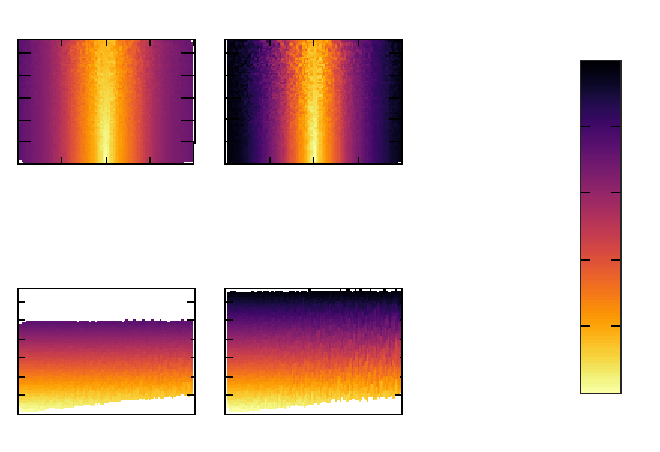
\includegraphics{./figures/parts/03/chapters/02/sections/01/caer_pf}}%
    \gplfronttext
  \end{picture}%
\endgroup

  \vspace{1cm}
  \caption{\small Κατόψεις (πρώτη σειρά) και πλάγιες όψεις
           (δεύτερη σειρά) της μετρικής CAER (εξίσωση \ref{eq:caer_normal}) από
           $10^5$ ζεύγη μίας σάρωσης σταθερής στάσης και εικονικών σαρώσεων που
           συνελήφθησαν από τυχαίες στάσεις, ανάλογα με την απόσταση $\|\Delta
           \bm{l}\|_2 = (\Delta x^2 + \Delta y^2)^{1/2}$, $\Delta x, \Delta y
           \in [-0.2, +0,2]$ m, και το σχετικού προσανατολισμό $\Delta \theta
           \in [-\pi/, +\pi/4]$ rad των στάσεων από όπου αυτές καταγράφηκαν,
           για αισθητήρες με εύρος $\lambda = 3\pi/2$ rad (αριστερή στήλη) και
           $\lambda = \pi$ rad (δεξιά). Οι εκτιμήσεις στάσεων που είναι πιο
           κοντά στην πραγματική στάση από άποψη (α) προσανατολισμού και (β)
           θέσης παρουσιάζουν χαμηλότερες τιμές CAER από εκείνες που απέχουν
           περισσότερο από αυτήν---: η μετρική CAER ικανοποιεί τα κριτήρια Κ1
           και Κ2 ακόμα και για μη πανοραμικούς
           αισθητήρες (ενότητα \ref{subsection:02_04_04:01})}
  \label{fig:03_02_01:caer}
\end{figure}
